\documentclass[a4paper,11pt]{ltjsarticle}
\usepackage[margin=18mm]{geometry}
\usepackage{amsmath}
\usepackage{graphicx}
\usepackage{fancyvrb}
\usepackage{float}

\graphicspath{{../}}
\fvset{frame=single, fontsize=\footnotesize, numbers=left, numbersep=4pt, framesep=2mm, samepage=true}

\newcommand{\conc}[1]{[\mathrm{#1}]}
\newcommand{\dd}[2]{\frac{d#1}{d#2}}

\pagestyle{plain}

\begin{document}

\begin{center}
  {\Large 第1回 宿題　常微分方程式と生化学反応系}\par\medskip
  学籍番号 \underline{\hspace{40mm}}\quad 氏名 \underline{\hspace{50mm}}
\end{center}

\section*{演習1　生化学反応系の微分方程式を書き下ろす}
反応系 $S_1 \xrightarrow{v_1} S_2 \xrightarrow{v_2} \phi$ について答える。

\paragraph{1.}
質量作用の法則より，反応速度式は
\[
  v_1 = k_1 \conc{S_1}, \qquad v_2 = k_2 \conc{S_2}.
\]

\paragraph{2.}
$S_2$ は反応 $v_1$ で生成し，反応 $v_2$ で消費されるので，
\[
  \dd{\conc{S_2}}{t} = v_1 - v_2 = k_1 \conc{S_1} - k_2 \conc{S_2}.
\]

\section*{演習2　生化学反応系の微分方程式を変数分離法で解く}
以下，$\conc{Glc} = \conc{Glucose}$ と略記する。

\paragraph{1.}
微分方程式 $\displaystyle \dd{\conc{Glc}}{t} = -k\conc{Glc}$ の両辺を $\conc{Glc}$ で割り，$t$ で積分すると
\begin{align*}
  \int \frac{d\conc{Glc}}{\conc{Glc}} &= \int (-k)\, dt \\
  \log \conc{Glc} &= -kt + C \qquad (C \text{ は積分定数}) \\
  \conc{Glc} &= e^{-kt + C} = e^{C} e^{-kt} = C' e^{-kt} \qquad (C' = e^{C}).
\end{align*}
初期条件 $\conc{Glc}(t=0) = 1.0\ \mathrm{mM}$ より
\[
  \conc{Glc}(0) = C' e^{0} = C' = 1.0\ \mathrm{mM}.
\]
よって
\[
  \conc{Glc}(t) = 1.0\, e^{-kt}\ \mathrm{mM}.
\]

\paragraph{2.}
$k = 0.2\ \mathrm{sec^{-1}}$ のとき $\conc{Glc}(t) = 1.0\, e^{-0.2t}\ \mathrm{mM}$ である。
$t = 0$ 〜 $5.0\ \mathrm{sec}$ の範囲を matplotlib で描いた（図\ref{fig:analytic}）。

\begin{figure}[H]
  \begin{minipage}[c]{0.47\linewidth}
    \VerbatimInput[label={glucose\_analytic.py}]{../glucose_analytic.py}
  \end{minipage}\hfill
  \begin{minipage}[c]{0.45\linewidth}
    \centering
    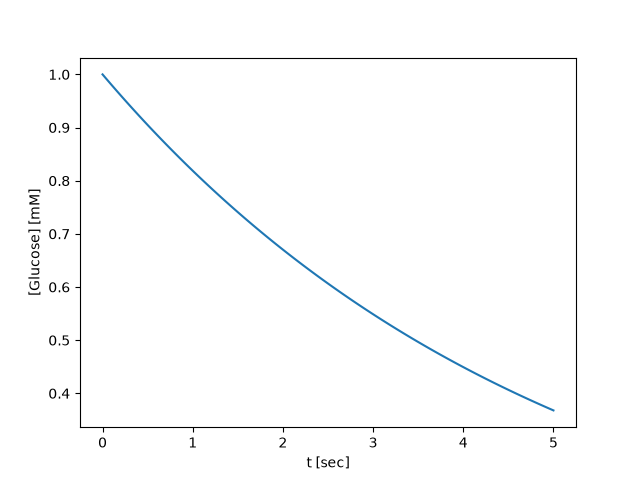
\includegraphics[width=\linewidth]{glucose_analytic.png}
  \end{minipage}
  \caption{glucose\_analytic.py（左）と解析解 $\conc{Glc}(t) = 1.0\, e^{-0.2t}$ のグラフ（右）}
  \label{fig:analytic}
\end{figure}

\section*{演習3　オイラー法で微分方程式の数値解を求める}

\paragraph{1.}
オイラー法の更新式
\[
  \conc{Glc}(t + \Delta t) = \conc{Glc}(t) + \Delta t \cdot \bigl(-k \conc{Glc}(t)\bigr)
\]
に合わせて，euler\_matplotlib.py の速度定数を \texttt{k = -0.2}（$-k$ に相当），
終了時刻を \texttt{endtime = 5.0} に書き換えた。
初期値は \texttt{y = 1.0}（mM），刻み幅は \texttt{delta\_t = 0.01}（sec）のままである。

\paragraph{2.}
コードと実行結果を図\ref{fig:euler}に示す。

\begin{figure}[H]
  \begin{minipage}[c]{0.47\linewidth}
    \VerbatimInput[label={euler\_matplotlib.py}]{../euler_matplotlib.py}
  \end{minipage}\hfill
  \begin{minipage}[c]{0.45\linewidth}
    \centering
    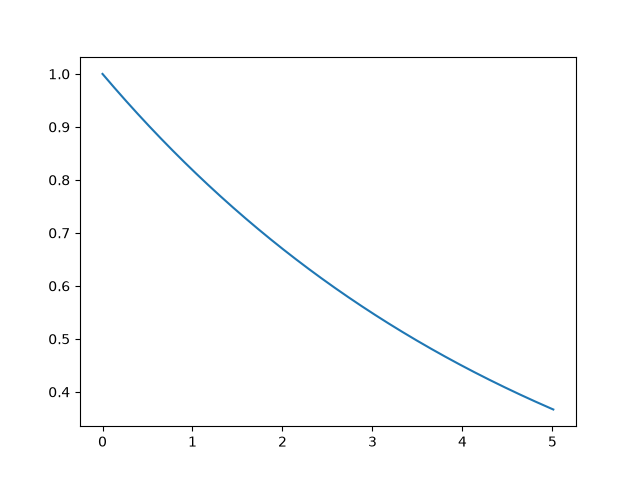
\includegraphics[width=\linewidth]{euler_matplotlib.png}
  \end{minipage}
  \caption{euler\_matplotlib.py（左）とオイラー法による $\conc{Glc}(t)$ の数値解（右。横軸 $t$ [sec]，縦軸 $\conc{Glc}$ [mM]）}
  \label{fig:euler}
\end{figure}

\section*{演習4　solve\_ivp を用いた生化学反応系のシミュレーション}
反応系 $S_1 \xrightarrow{v_1} S_2 \xrightarrow{v_2} \phi$，
$\displaystyle v_1 = \frac{V_{m1}\conc{S_1}}{K_{m1} + \conc{S_1}}$，
$\displaystyle v_2 = \frac{V_{m2}\conc{S_2}}{K_{m2} + \conc{S_2}}$ について答える。

\paragraph{1.}
$S_1$ は $v_1$ で消費され，$S_2$ は $v_1$ で生成し $v_2$ で消費されるので，
\begin{align*}
  \dd{\conc{S_1}}{t} &= -v_1 = -\frac{V_{m1}\conc{S_1}}{K_{m1} + \conc{S_1}}, \\
  \dd{\conc{S_2}}{t} &= v_1 - v_2 = \frac{V_{m1}\conc{S_1}}{K_{m1} + \conc{S_1}} - \frac{V_{m2}\conc{S_2}}{K_{m2} + \conc{S_2}}.
\end{align*}

\paragraph{2.}
空欄は「1」の式に合わせて \verb|v2 = Vmax2 * S2 / ( Km2 + S2 )|，\verb|ds2dt = v1 - v2| と埋めた（10，14 行目）。
コード全体と実行結果（図\ref{fig:michaelis}）を示す。

\VerbatimInput[label={michaelis.py}]{../michaelis.py}

\begin{figure}[H]
  \centering
  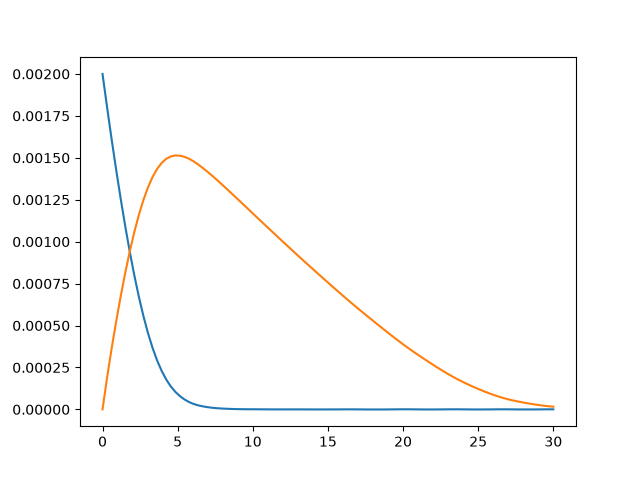
\includegraphics[width=0.5\linewidth]{michaelis.png}
  \caption{solve\_ivp による数値解。青線が $\conc{S_1}$，橙線が $\conc{S_2}$（横軸は時間 $t$，縦軸は濃度）}
  \label{fig:michaelis}
\end{figure}

\end{document}
